\documentclass[11pt,dvipsnames,cmyk]{article}

\usepackage{listings}
\usepackage{xcolor}
\usepackage[utf8]{inputenc}
\usepackage[a4paper, margin=1in]{geometry}
\usepackage{graphicx}

\lstdefinestyle{sharpc}{language=[Sharp]C,
morekeywords={Object}}
\lstdefinestyle{vb}{language=[Visual]Basic,
morekeywords={As,Boolean,Byte,Char,Double,Imports,Module,New,Single}}

\pagenumbering{gobble}
\renewcommand{\theenumi}{\roman{enumi}}
\setlength{\tabcolsep}{48pt}

\title{Lab Assignment}
\author{Sudhanshu Kumar\\
2017IEN43\\
Department of Computer Science}

\begin{document}
	\maketitle
	\break
	\section*{Explain the concept of boxing and unboxing in C\# with an example.}
	C\# Type System contains three Types, they are \emph{Value Types}, \emph{Reference Types} and \emph{Pointer Types}. In C\# it is possible to convert a value of one type into a value of another type. C\# allows us to convert a Value Type to a Reference Type, and back again to Value Types. The operation of converting a \emph{Value Type} to a \emph{Reference Type} is called \emph{Boxing} and the reverse operation is called \emph{Unboxing}.
	\lstset{style=sharpc}
	\begin{lstlisting}
	int Val = 1;
	Object Obj = Val;	//Boxing
	int i = (int)Obj;	//Unboxing
	\end{lstlisting}
	From the above operation (Object Obj = i) we saw converting a value of a Value Type into a value of a corresponding Reference Type. These types of operation is called \emph{Boxing}. The next line (int i = (int) Obj) shows extracts the Value Type from the Object. That is converting a value of a Reference Type into a value of a Value Type. This operation is called \emph{Unboxing}.
	\\\emph{Boxing} and \emph{Unboxing} are computationally expensive processes. When a value type is boxed, an entirely new object must be allocated and constructed, also the cast required for unboxing is also expensive computationally.\\\\\\
	\rule{6.27in}{1.2pt}
	
	\section*{Explain the basic program structure in VB.NET.}
	A VB.Net program basically consists of the following parts ---
	\begin{itemize}
		\item Namespace declaration
		\item A class or module
		\item One or more procedures
		\item Variables
		\item The Main procedure
		\item Statements \& Expressions
		\item Comments
	\end{itemize}
	Let us look at a simple code that would print the words "Hello World" ---
	\lstset{style=vb}
	\begin{lstlisting}
	Imports System
	
	Module Program
		'This program displays Hello World!
		Sub Main(args As String())
			Console.WriteLine("HelloWorld!")
			Console.ReadKey()
		End Sub
	End Module
	\end{lstlisting}
	When the above code is compiled and executed, it produces the following result ---
	\begin{verbatim}
	Hello World!
	\end{verbatim}
	Let us look various parts of the above program ---
	\begin{itemize}
		\item The first line of the program \textbf{Imports System} is used to include the \emph{System} namespace in the program.
		
		\item The next line has a Module declaration, the module \textbf{Program}. VB.Net is completely object oriented, so every program must contain a module of a class that contains the data and procedures that your program uses.
		
		\item Classes or Modules generally would contain more than one procedure. Procedures contain the executable code, or in other words, they define the behavior of the class. A procedure could be any of the following ---
		\begin{itemize}
			\item Function
			\item Sub
			\item Operator
			\item Get
			\item Set
			\item AddHandler
			\item RemoveHandler
			\item RaiseEvent
		\end{itemize}
		
		\item The next line \emph{('This program)} will be ignored by the compiler and it has been put to add additional comments in the program.
		
		\item The next line defines the \textbf{Main} procedure, which is the entry point for all VB.Net programs. The \emph{Main} procedure states what the module or class will do when executed.
		
		\item The \emph{Main} procedure specifies its behavior with the statement.
		
		\item \textbf{Console.WriteLine("Hello World!")} \emph{WriteLine} is a method of the Console class defined in the \emph{System} namespace. This statement causes the message \emph{"Hello World!"} to be displayed on the screen.
		
		\item The last line \textbf{Console.ReadKey()} is for the VS.NET Users. This will prevent the screen from running and closing quickly when the program is launched from Visual Studio .NET.
	\end{itemize}	
	\hfill\break\rule{6.27in}{1.2pt}
	
	\section*{Explain the following related to VB.NET programming.
		\begin{enumerate}
			\item Data types and declaring a variable.
			\item Directives
			\item Creating a sub procedure.
			\item Creating objects and classes
		\end{enumerate}}
	
	\textbf{Data types and declaring a variable}\\
	Data types refer to an extensive system used for declaring variables or functions of different types. The type of a variable determines how much space it occupies in storage and how the bit pattern stored is interpreted.\\The following table shows some of the data types available ---
	\begin{center}
		\begin{tabular}{||c c||}
			\hline\hline
			Data Type & Storage Allocation\\
			\hline
			Byte & 1 Byte\\
			\hline
			Char & 2 Bytes\\
			\hline
			Date & 8 Bytes\\
			\hline
			Decimal & 16 Bytes\\
			\hline
			Double & 8 Bytes\\
			\hline
			Integer & 4 Bytes\\
			\hline
			Long & 8 Bytes\\
			\hline
			Short & 2 Bytes\\
			\hline\hline
		\end{tabular}
	\end{center}
	A variable is nothing but a name given to a storage area that our programs can manipulate. Each variable in VB.Net has a specific type, which determines the size and layout of the variable's memory; the range of values that can be stored within that memory; and the set of operations that can be applied to the variable. The \textbf{Dim} statement is used for variable declaration and storage allocation for one or more variables. The \emph{Dim} statement is used at module, class, structure, procedure or block level. The following codes demonstrates declaration of some of the types ---
	\begin{lstlisting}
	Dim b As Byte
	Dim c As Char
	Dim StudentID As Integer
	Dim StudentName As String
	Dim Salary As Double
	Dim count1, count2 As Integer
	Dim status As Boolean
	Dim exitButton As New System.Windows.Forms.Button
	Dim lastTime, nextTime As Date
	\end{lstlisting}
	You can initialize a variable at the time of declaration as follows ---
	\begin{lstlisting}
	Dim StudentID As Integer = 100
	Dim StudentName As String = "BillSmith"
	\end{lstlisting}
	
	\hfill\break\textbf{Directives}\\
	The VB.Net compiler directives give instructions to the compiler to preprocess the information before actual compilation starts. All these directives begin with \#, and only white-space characters may appear before a directive on a line. These directives are not statements. VB.Net compiler does not have a separate preprocessor; however, the directives are processed as if there was one. In VB.Net, the compiler directives are used to help in conditional compilation.\\
	VB.Net provides the following set of compiler directives ---
	\begin{itemize}
		\item \textbf{The \#Const Directive}\\
		This directive defines conditional compiler constants.
		\begin{verbatim}
		#Const state = "WEST BENGAL"
		\end{verbatim}
		
		\item \textbf{The \#ExternalSource Directive}\\
		This directive is used for indicating a mapping between specific lines of source code and text external to the source. It is used only by the compiler and the debugger has no effect on code compilation. This directive allows including external code from an external code file into a source code file.
		\begin{verbatim}
		#ExternalSource("c:\vbprogs\directives.vb", 5)
		Console.WriteLine("This is External Code. ")
		#End ExternalSource
		\end{verbatim}
		
		\item \textbf{The \#If...Then...\#Else Directives}\\
		This directive conditionally compiles selected blocks of Visual Basic code.
		\begin{verbatim}
		#Const TargetOS = "Linux"
		#If TargetOS = "Windows 7" Then
		' Windows 7 specific code
		#ElseIf TargetOS = "WinXP" Then
		' Windows XP specific code
		#Else
		' Code for other OS
		#End if
		\end{verbatim}
		
		\item \textbf{The \#Region Directive}\\
		This directive helps in collapsing and hiding sections of code in Visual Basic files.
		\begin{verbatim}
		#Region "StatsFunctions" 
		' Insert code for the Statistical functions here.
		#End Region
		\end{verbatim}
	 \end{itemize}
 
	 \hfill\break\textbf{Creating a sub procedure}\\
	 Sub procedures are procedures that do not return any value. We have been using the Sub procedure Main in all our examples. When the applications start, the control goes to the Main Sub procedure, and it in turn, runs any other statements constituting the body of the program. The Sub statement is used to declare the name, parameter and the body of a sub procedure. The syntax for the Sub statement is ---
	 \begin{verbatim}
	 [Modifiers] Sub SubName [(ParameterList)] 
	 [Statements]
	 End Sub
	 \end{verbatim}
	 Where,
	 \begin{itemize}
	 	\item  \textbf{Modifiers} specify the access level of the procedure; possible values are - \emph{Public, Private, Protected, Friend, Protected Friend} and information regarding \emph{overloading, overriding, sharing} and \emph{shadowing.}
	 	
	 	\item \textbf{SubName} indicates the name of the Sub.
	 	
	 	\item \textbf{ParameterList} specifies the list of the parameters.
	 \end{itemize}
	 Example---\begin{verbatim}
	 Sub CalculatePay(ByRef hours As Double, ByRef wage As Decimal)
	 'local variable declaration
	 Dim pay As Double
	 pay = hours * wage
	 Console.WriteLine("Total Pay: {0:C}", pay)
	 End Sub
	 \end{verbatim}
	 
	 \hfill\break\textbf{Creating objects and classes}\\
	 When you define a class, you define a blueprint for a data type. This doesn't actually define any data, but it does define what the class name means, that is, what an object of the class will consist of and what operations can be performed on such an object. Objects are instances of a class. The methods and variables that constitute a class are called members of the class.\\
	 A typical declaration of class is ---
	 \begin{verbatim}
	 Class Box
	 Public length As Double    ' Length of a box
	 Public breadth As Double   ' Breadth of a box
	 Public height As Double    ' Height of a box
	 
	 Public Sub setLength(ByVal len As Double)
	 length = len
	 End Sub
	 
	 Public Sub setBreadth(ByVal bre As Double)
	 breadth = bre
	 End Sub
	 
	 Public Sub setHeight(ByVal hei As Double)
	 height = hei
	 End Sub
	 
	 Public Function getVolume() As Double
	 Return length * breadth * height
	 End Function
	 
	 End Class
	 \end{verbatim}
	 Objects can be declared as ---
	 \begin{verbatim}
	 	Dim Box1 As Box = New Box()        ' Declare Box1 of type Box
	 	Dim Box2 As Box = New Box()        ' Declare Box2 of type Box
	 \end{verbatim}
	 \hfill\break\rule{6.27in}{1.2pt}
	 
	 \section*{Briefly discuss the 6 types of access modifiers supported in C\# with an example program.}
	 \emph{Access Modifiers ( Access Specifiers )} describes as the scope of accessibility of an Object and its members. All C\# types and type members have an accessibility level . We can control the scope of the member object of a class using access specifiers. We are using access modifiers for providing security of our applications. When we specify the accessibility of a type or member we have to declare it by using any of the access modifiers provided by C\# language.
	 \\C\# provide six access modifiers , they are as follows ---
	 \begin{itemize}
	 	\item \textbf{Private Access Modifier}
	 	\\The scope of the accessibility is limited only inside the \emph{classes} or \emph{struct} in which they are declared. The private members cannot be accessed outside the class and it is the least permissive access level.
	 	\\Example ---
	 	\begin{verbatim}
	 	using System;
	 	namespace ConsoleApplication1
	 	{
	 	class Program
	 	{
	 	private string msg = "This variable is private ";
	 	private void disp(string msg)
	 	{
	 	Console.WriteLine("This function is private : " + msg);
	 	}
	 	static void Main(string[] args)
	 	{
	 	Program pr = new Program();
	 	Console.WriteLine(pr.msg);	//Accessing private variable  inside the class
	 	pr.disp("Hello !!");  //Accessing private function  inside the class
	 	}
	 	}
	 	}
	 	\end{verbatim}
	 	Output ---
	 	\begin{verbatim}
	 	This variable is private
	 	This function is private : Hello !!
	 	\end{verbatim}
	 	
	 	\item \textbf{Public Access Modifier}
	 	\\This is the most common access specifier in C\# . It can be accessed from anywhere, that means there is no restriction on accessibility. The scope of the accessibility is inside \emph{class} as well as outside. The type or member can be accessed by any other code in the same assembly or another assembly that references it.
	 	\\Example ---
	 	\begin{verbatim}
	 	using System;
	 	namespace ConsoleApplication1
	 	{
	 	class PublicAccess
	 	{
	 	public string msg = "This variable is public";
	 	public void disp(string msg)
	 	{
	 	Console.WriteLine("This function is public : " + msg);
	 	}
	 	}
	 	class Program
	 	{
	 	static void Main(string[] args)
	 	{
	 	PublicAccess pAccess = new PublicAccess();
	 	Console.WriteLine(pAccess.msg); // Accessing public variable
	 	pAccess.disp("Hello !!"); // Accessing public function
	 	}
	 	}
	 	}
	 	\end{verbatim}
	 	Output ---
	 	\begin{verbatim}
	 	This variable is public
	 	This function is public : Hello !!
	 	\end{verbatim}
	 	
	 	\item \textbf{Protected Access Modifier}
	 	\\The scope of accessibility is limited within the \emph{class} or \emph{struct} and the class derived from this class.
	 	\\Example ---
	 	\begin{verbatim}
	 	using System;
	 	namespace ConsoleApplication1
	 	{
	 	class ProtectedAccess
	 	{
	 	protected string msg = "This variable is protected  ";
	 	protected void disp(string msg)
	 	{
	 	Console.WriteLine("This function is protected : " + msg);
	 	}
	 	}
	 	class Program : ProtectedAccess	//Derived class
	 	{
	 	static void Main(string[] args)
	 	{
	 	Program pr = new Program();
	 	Console.WriteLine(pr.msg); // Accessing protected variable
	 	pr.disp("Hello !!");  // Accessing protected function
	 	}
	 	}
	 	}
	 	\end{verbatim}
	 	
	 	\item \textbf{Internal Access Modifier}
	 	\\The internal access modifiers can access within the program that contain its declarations and also access only within files in the same assembly level but not from another assembly.
	 	\\Example ---
	 	\begin{verbatim}
	 	using System;
	 	namespace ConsoleApplication1
	 	{
	 	class InternalAccess
	 	{
	 	internal string msg = "This variable is internal";
	 	internal void disp(string msg)
	 	{
	 	Console.WriteLine("This function is internal : " + msg);
	 	}
	 	}
	 	class Program
	 	{
	 	static void Main(string[] args)
	 	{
	 	InternalAccess iAccess = new InternalAccess();
	 	Console.WriteLine(iAccess.msg); // Accessing internal variable
	 	iAccess.disp("Hello !!"); // Accessing internal function
	 	Console.ReadKey();
	 	}
	 	}
	 	}
	 	\end{verbatim}
	 	Output ---
	 	\begin{verbatim}
	 	This variable is internal
	 	This function is internal : Hello !!
	 	\end{verbatim}
	 	
	 	\item \textbf{Protected Internal Access Modifier}
	 	\\Protected internal is the same access levels of both protected and internal . It can access anywhere in the same assembly also be accessed within a derived class in another assembly.
	 	\\Example ---
	 	\begin{verbatim}
	 	using System;
	 	namespace ConsoleApplication1
	 	{
	 	class InternalAccess
	 	{
	 	protected internal string msg = "This variable is  protected internal";
	 	protected internal void disp(string msg)
	 	{
	 	Console.WriteLine("This function is protected internal : " + msg);
	 	}
	 	}
	 	class Program
	 	{
	 	static void Main(string[] args)
	 	{
	 	InternalAccess iAccess = new InternalAccess();
	 	Console.WriteLine(iAccess.msg); // Accessing internal variable
	 	iAccess.disp("Hello !!"); // Accessing internal function
	 	Console.ReadKey();
	 	}
	 	}
	 	}
	 	\end{verbatim}
	 	Output ---
	 	\begin{verbatim}
	 	This variable is  protected internal
	 	This function is protected internal : Hello !!
	 	\end{verbatim}
	 	
	 	\item \textbf{Private Protected Access Modifier}
	 	\\The new modifier private protected really means \emph{protected and also internal.} That is, member is accessible only to child classes which are in the same assembly, but not to child classes which are outside assembly.That is useful if you build hierarchy of classes in your assembly and do not want any child classes from other assemblies to access certain parts of that hierarchy.
	 	\\Example ---\\
	 	\begin{verbatim}
	 	Assembly1.cs
	 	// Compile with: /target:library
	 	public class MyBaseClass
	 	{
	 	private protected int count = 0;
	 	}
	 	public class MyDerivedClass1 : MyBaseClass
	 	{
	 	void callMe()
	 	{
	 	MyBaseClass obj = new MyBaseClass();
	 	obj.count = 5;
	 	// Error CS1540, because the variable count can only be accessed by
	 	// classes derived from MyBaseClass.
	 	count = 5; // OK, accessed through the current derived class instance
	 	}
	 	}
	 	\end{verbatim}
	 	\begin{verbatim}
	 	Assembly2.cs
	 	// Compile with: /reference:Assembly1.dll
	 	class MyDerivedClass2 : MyBaseClass
	 	{
	 	void callMe()
	 	{
	 	count = 10;
	 	// Error CS0122, because count can only be
	 	// accessed by types in Assembly1
	 	}
	 	}
	 	\end{verbatim}
	 	
	 	\item \textbf{Default access modifiers in C\#}
	 	\\When no access modifier is set, a default access modifier is used. So there is always some form of access modifier even if it's not set. The default access for everything in C\# is "the most restricted access you could declare for that member".
	 	
	 	\item \textbf{Static modifier}
	 	\\The static modifier on a class means that the class cannot be instantiated, and that all of its members are static. A static member has one version regardless of how many instances of its enclosing type are created.
	 	
	 \end{itemize}
	 \rule{6.27in}{1.2pt}
	 
	 \section*{Explain any 4 types of C\# collections with an example.}
	 \begin{enumerate}
	 	\item \textbf{ArrayList}
	 	\begin{itemize}
	 		\item The Add() method of ArrayList is used to add new items in ArrayList.
	 		\begin{verbatim}
	 		ArrayList.Add(object)
	 		\end{verbatim}
	 		\item ArrayList Insert(Int32, Object) method inserts an element into the ArrayList at the specified index.
	 		\begin{verbatim}
	 		ArrayList.Insert(index,object)
	 		\end{verbatim}
	 		\item Arraylist remove() method removes the first occurrence of a specific object from the ArrayList.
	 		\begin{verbatim}
	 		ArrayList.Remove(object)
	 		\end{verbatim}
	 		\item\emph{ArrayList.RemoveAt(index)} remove the specified index element from arraylist.\\
	 		\item\emph{ArrayList.RemoveRange(Int32, Int32)} method is used to remove a range of elements from the ArrayList.\\
	 		\item Arraylist Sort() method sorts the elements in the entire ArrayList.
	 		\begin{verbatim}
	 		ArrayList.Sort()
	 		\end{verbatim}
	 	\end{itemize}
 		\begin{verbatim}
 		namespace ConsoleApplication1
 		{
 		class Program
 		{
 		static void Main(string[] args)
 		{
 		ArrayList arrList = new ArrayList();
 		arrList.Add("North");
 		arrList.Add("West");
 		arrList.Add("South");
 		Console.WriteLine("ArrayList Elements...");
 		foreach (object item in arrList)
 		{
 		Console.WriteLine(item);
 		}
 		
 		//insert an item at the top of arraylist
 		arrList.Insert(0, "Directions");
 		//insert an item at the 3rd position  of arraylist
 		arrList.Insert(2, "East");
 		Console.WriteLine("ArrayList Elements after insert...");
 		foreach (object item in arrList)
 		{
 		Console.WriteLine(item);
 		}
 		
 		//remove() method removes the first occurrence
 		arrList.Remove("West");
 		Console.WriteLine("ArrayList Elements after remove()...");
 		foreach (object item in arrList)
 		{
 		Console.WriteLine(item);
 		}
 		arrList.Insert(3,"West");
 		//remove element at index 1
 		arrList.RemoveAt(1);
 		Console.WriteLine("ArrayList Elements after removeAt()...");
 		foreach (object item in arrList)
 		{
 		Console.WriteLine(item);
 		}
 		arrList.Insert(1,"North");
 		
 		//remove range of elements from arraylist
 		arrList.RemoveRange(1,2);
 		Console.WriteLine("ArrayList Elements after RemoveRange()...");
 		foreach (object item in arrList)
 		{
 		Console.WriteLine(item);
 		}
 		arrList.Insert(1,"North");
 		arrList.Insert(2,"East");
 		
 		//sort arraylist elements
 		arrList.Sort();
 		Console.WriteLine("ArrayList Elements after sort()...");
 		foreach (object item in arrList)
 		{
 		Console.WriteLine(item);
 		}
 		Console.ReadKey();
 		}
 		}
 		}
 		\end{verbatim}
 		\item\textbf{HashTable}
 		\\Hashtable in C\# represents a collection of key/value pairs which maps keys to value. Any non-null object can be used as a key but a value can. We can retrieve items from hashTable to provide the key . Both keys and values are Objects.
 		\\The commonly used functions in Hashtable are ---
 		\begin{itemize}
 			\item \emph{Add} : To add a pair of value in HashTable
 			\begin{verbatim}
 			HashTable.Add(Key,Value)
 			\end{verbatim}
 			\item \emph{ContainsKey} : Check if a specified key exist or not
 			\begin{verbatim}
 			bool HashTable.ContainsKey(key)
 			\end{verbatim}
 			\item \emph{ContainsValue} : Check the specified Value exist in HashTable
 			\begin{verbatim}
 			bool HashTable.ContainsValue(Value)
 			\end{verbatim}
 			\item \emph{Remove} : Remove the specified Key and corresponding Value
 			\begin{verbatim}
 			HashTable.Remove(Key)
 			\end{verbatim}
 		\end{itemize}
		\begin{verbatim}
		namespace WindowsApplication1
		{
		public partial class Form1 : Form
		{
		public Form1()
		{
		InitializeComponent();
		}
		
		private void button1_Click(object sender, EventArgs e)
		{
		Hashtable weeks = new Hashtable();
		weeks.Add("1", "SunDay");
		weeks.Add("2", "MonDay");
		weeks.Add("3", "TueDay");
		weeks.Add("4", "WedDay");
		weeks.Add("5", "ThuDay");
		weeks.Add("6", "FriDay");
		weeks.Add("7", "SatDay");
		//Display a single Item 
		
		MessageBox.Show(weeks["5"].ToString ());
		//Search an Item 
		if (weeks.ContainsValue("TueDay"))
		{
		MessageBox.Show("Find");
		}
		else
		{
		MessageBox.Show("Not find");
		}
		//remove an Item 
		weeks.Remove("3");
		//Display all key value pairs
		foreach (DictionaryEntry day in weeks )
		{
		MessageBox.Show (day.Key + "  " + day.Value );
		}
		}
		}
		}
		\end{verbatim}
		
		\item \textbf{Stack}
		\\The \emph{Stack class} represents a last-in-first-out (LIFO) Stack of Objects. Stack is implemented as a circular buffer. It follows the Last In First Out (LIFO) system. That is we can push the items into a stack and get it in reverse order. Stack returns the last item first. As elements are added to a Stack, the capacity is automatically increased as required through reallocation.
		\\Commonly used methods ---
		\begin{itemize}
			\item \emph{Push} : Add (Push) an item in the Stack data structure
			\begin{verbatim}
			Stack.Push(Object)
			\end{verbatim}
			\item \emph{Pop} : Pop return the last Item from the Stack
			\begin{verbatim} 
			Object Stack.Pop()			
			\end{verbatim}
			\item \emph{Contains} : Check the object contains in the Stack
			\begin{verbatim} 
			Stack.Contains(Object)			
			\end{verbatim}
		\end{itemize}
		\begin{verbatim}
		using System;
		using System.Collections;
		using System.ComponentModel;
		using System.Data;
		using System.Drawing;
		using System.Text;
		using System.Windows.Forms;
		
		namespace WindowsApplication1
		{
		public partial class Form1 : Form
		{
		public Form1()
		{
		InitializeComponent();
		}
		
		private void button1_Click(object sender, EventArgs e)
		{
		Stack days = new Stack();
		days.Push("SunDay");
		days.Push("MonDay");
		days.Push("TueDay");
		days.Push("WedDay");
		days.Push("ThuDay");
		days.Push("FriDay");
		days.Push("SaturDay");
		if (days.Count ==7)
		{
		MessageBox.Show(days.Pop().ToString ());
		}
		else
		{
		MessageBox.Show("SaturDay does not exist");
		}
		}
		}
		}
		\end{verbatim}
 		
 		\item \textbf{Queue}
 		\\The Queue works like FIFO system , a first-in, first-out collection of Objects. Objects stored in a Queue are inserted at one end and removed from the other. The Queue provide additional insertion, extraction, and inspection operations. We can Enqueue (add) items in Queue and we can Dequeue (remove from Queue ) or we can Peek (that is we will get the reference of first item ) item from Queue. Queue accepts null reference as a valid value and allows duplicate elements.
 		\\Some important functions in the Queue Class are follows :
 		\begin{itemize}
 			\item \emph{Enqueue} : Add an Item in Queue
 			\begin{verbatim}
 			Queue.Enqueue(Object)
 			\end{verbatim}
 			\item \emph{Dequeue} : Remove the oldest item from Queue
 			\begin{verbatim}
 			Object Queue.Dequeue()
 			\end{verbatim}
 			\item \emph{Peek} : Get the reference of the oldest item
 			\begin{verbatim}
 			Object Queue.Peek()
 			\end{verbatim}
 		\end{itemize}
 		\begin{verbatim}
 		using System;
 		using System.Collections;
 		using System.Windows.Forms;
 		
 		namespace WindowsApplication1
 		{
 		public partial class Form1 : Form
 		{
 		public Form1()
 		{
 		InitializeComponent();
 		}
 		
 		private void button1_Click(object sender, EventArgs e)
 		{
 		Queue days = new Queue();
 		days.Enqueue("Sunday");
 		days.Enqueue("Monday");
 		days.Enqueue("Tuesday");
 		days.Enqueue("Wednsday");
 		days.Enqueue("Thursday");
 		days.Enqueue("Friday");
 		days.Enqueue("Saturday");
 		
 		MessageBox.Show (days.Dequeue().ToString ());
 		
 		if (days.Contains("Monday"))
 		{
 		MessageBox.Show("The queue contains Monday");
 		}
 		else
 		{
 		MessageBox.Show("Does not match any entries");
 		}
 		}
 		}
 		}
 		\end{verbatim}
	 \end{enumerate}
 	 \rule{6.27in}{1.2pt}
 	 
 	 \section*{How to create a PDF file from text file using C\# ? Write a program to implement the same.}
	 Pdfsharp is a popular open source framework which could be used to create PDF files programmatically. In many situations we need PDF documents instead of text documents because text files are listed as the simplest file format, which limits users only to edit words. From the following program you can easily convert a text file to a PDF formated document.
	 \lstset{style=sharpc}
	 \begin{verbatim}
	 using System;
	 using System.Windows.Forms;
	 using PdfSharp;
	 using PdfSharp.Drawing;
	 using PdfSharp.Pdf;
	 using System.Diagnostics;
	 using System.IO;
	 
	 namespace textToPdf
	 {
	 public partial class Form1 : Form
	 {
	 public Form1()
	 {
	 InitializeComponent();
	 }
	 
	 private void button1_Click(object sender, EventArgs e)
	 {
	 try
	 {
	 string line = null;
	 System.IO.TextReader readFile = new StreamReader("text.txt");
	 int yPoint = 0;
	 
	 PdfDocument pdf = new PdfDocument();
	 pdf.Info.Title = "txt to pdf";
	 PdfPage pdfPage = pdf.AddPage();
	 XGraphics graph = XGraphics.FromPdfPage(pdfPage);
	 XFont font = new XFont("Verdana", 20, XFontStyle.Regular);
	 
	 while (true)
	 {
	 line = readFile.ReadLine();
	 if (line == null)
	 {
	 break;
	 }
	 else
	 {
	 graph.DrawString(line, font, XBrushes.Black, new XRect(40, yPoint, pdfPage.Width.Point,
	  pdfPage.Height.Point), XStringFormats.TopLeft);
	 yPoint = yPoint + 40;
	 }
	 }
	 
	 string pdfFilename = "texttoPDF.pdf";
	 pdf.Save(pdfFilename);
	 readFile.Close();
	 readFile = null;
	 Process.Start(pdfFilename);
	 label1.text = "PDF generated";
	 }
	 
	 catch (Exception ex)
	 {
	 MessageBox.Show(ex.ToString());
	 }
	 }
	 }
	 }
	 \end{verbatim}
	 \begin{center}
	 	\textbf{Output}\\
	 	\hfill\break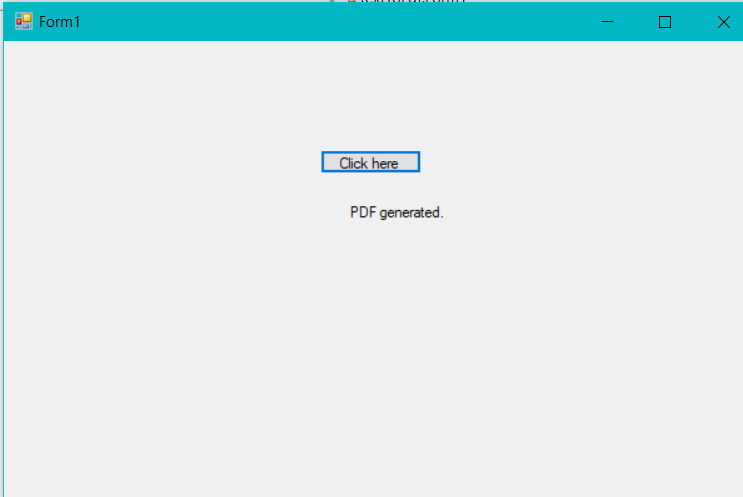
\includegraphics[width=4.27in]{6.png}
	 \end{center}
	 \rule{6.27in}{1.2pt}
	 
	 \section*{Write a C\# program to read and import excel file into dataset using OLEDB .}
	 \begin{verbatim}
	 using System;
	 using System.Data;
	 using System.Data.OleDb;
	 using System.Drawing;
	 using System.Windows.Forms;
	 
	 namespace excelToDatabase
	 {
	 public partial class Form1 : Form
	 {
	 public Form1()
	 {
	 InitializeComponent();
	 }
	 
	 private void button1_Click(object sender, EventArgs e)
	 {
	 try
	 {
	 OleDbConnection myConnection;
	 DataSet dataSet;
	 OleDbDataAdapter myCommand;
	 myConnection = new OleDbConnection("provider=Microsoft.Jet.OLEDB.4.0;Data
	  Source='file.xls';Extended Properties=Excel 8.0;");
	 myCommand = new OleDbDataAdapter("select * from [Sheet1$]", myConnection);
	 myCommand.TableMappings.Add("Table", "TestTable");
	 dataSet = new DataSet();
	 myCommand.Fill(dataSet);
	 dataGridView1.DataSource = dataSet.Tables[0];
	 myConnection.Close();
	 }
	 catch(Exception ex)
	 {
	 MessageBox.Show(ex.ToString());
	 }
	 }
	 }
	 }
	 \end{verbatim}
	 \begin{center}
	 	\textbf{Output}\\
	 	\hfill\break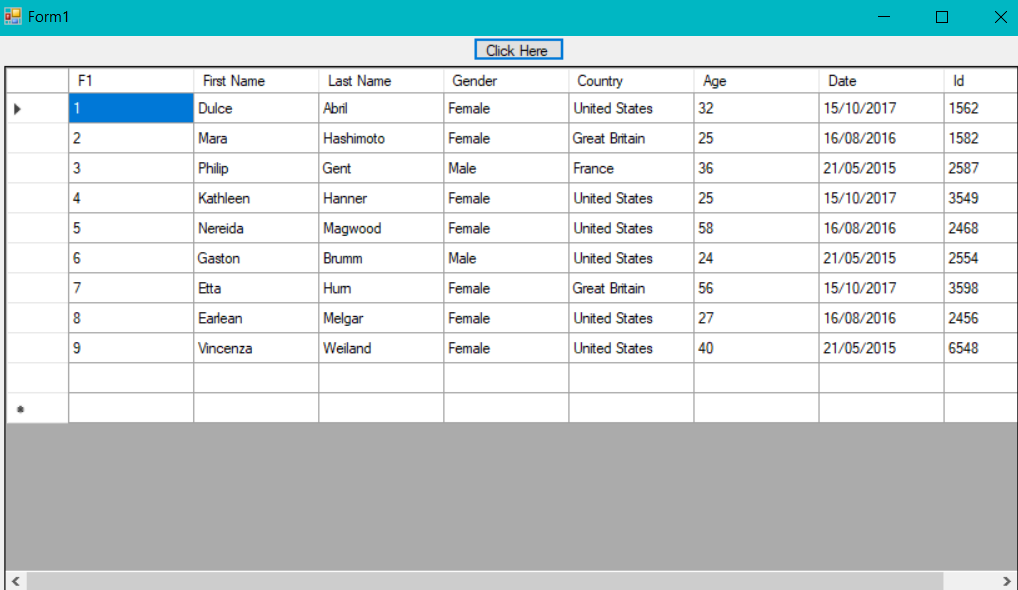
\includegraphics[width=4.27in]{7.png}
	 \end{center}
	 \rule{6.27in}{1.2pt}
	 
	 \section*{Write a Program to insert a data into excel file using OLEDB.}
	 \begin{verbatim}
	 using System;
	 using System.Data;
	 using System.Data.OleDb;
	 using System.Drawing;
	 using System.Windows.Forms;
	 
	 namespace insertData
	 {
	 public partial class Form1 : Form
	 {
	 public Form1()
	 {
	 InitializeComponent();
	 }
	 
	 private void button1_Click(object sender, EventArgs e)
	 {
	 try
	 {
	 OleDbConnection myConnection;
	 OleDbCommand myCommand = new OleDbCommand();
	 string sql = null;
	 myConnection = new OleDbConnection("provider=Microsoft.Jet.OLEDB.4.0;Data
	  Source='file.xls';Extended Properties=Excel 8.0;");
	 myConnection.Open();
	 myCommand.Connection = myConnection;
	 sql = "Insert into [Sheet1$] (id) values('25')";
	 myCommand.CommandText = sql;
	 myCommand.ExecuteNonQuery();
	 myConnection.Close();
	 label1.Text = "Inserted";
	 }
	 catch(Exception ex)
	 {
	 MessageBox.Show(ex.ToString());
	 }
	 }
	 }
	 }
	 \end{verbatim}
	 \begin{center}
	 	\textbf{Output}\\
	 	\hfill\break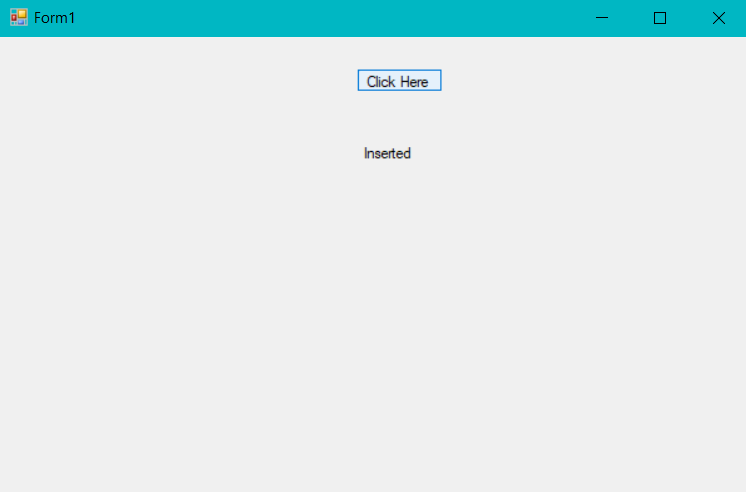
\includegraphics[width=4.27in]{8.png}
	 \end{center}
	 \rule{6.27in}{1.2pt}
	 
	 \section*{Write a program to update a data in an existing excel file using OLEDB.}
	 \begin{verbatim}
	 using System;
	 using System.Data;
	 using System.Data.OleDb;
	 using System.Drawing;
	 using System.Windows.Forms;
	 
	 namespace updateData
	 {
	 public partial class Form1 : Form
	 {
	 public Form1()
	 {
	 InitializeComponent();
	 }
	 
	 private void button1_Click(object sender, EventArgs e)
	 {
	 try
	 {
	 OleDbConnection myConnection;
	 OleDbCommand myCommand = new OleDbCommand();
	 string sql = null;
	 myConnection = new OleDbConnection("provider=Microsoft.Jet.OLEDB.4.0;Data
	  Source='file.xls';Extended Properties=Excel 8.0;");
	 myConnection.Open();
	 myCommand.Connection = myConnection;
	 sql = "Update [Sheet1$] set id = 23 where id=25";
	 myCommand.CommandText = sql;
	 myCommand.ExecuteNonQuery();
	 myConnection.Close();
	 label1.Text = "Updated";
	 }
	 catch(Exception ex)
	 {
	 MessageBox.Show(ex.ToString());
	 }
	 }
	 }
	 }
	 \end{verbatim}
	 \begin{center}
	 	\textbf{Output}\\
	 	\hfill\break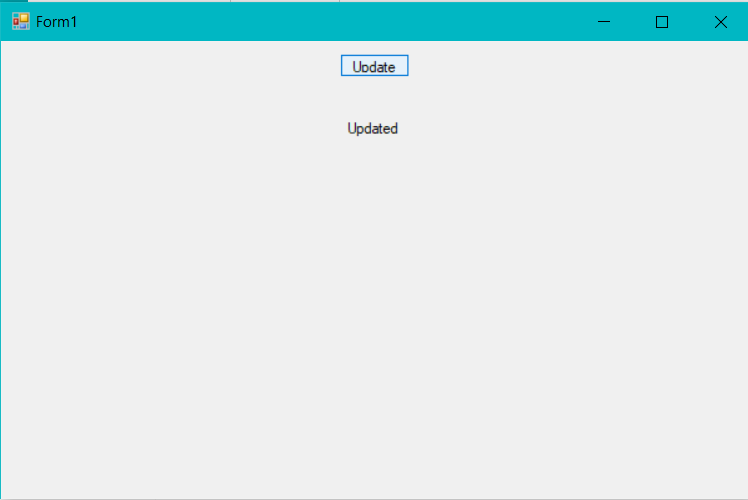
\includegraphics[width=4.27in]{9.png}
	 \end{center}
	 \rule{6.27in}{1.2pt}
	 
	 \section*{Write a program to send an email with attachment using C\# forms.}
	 \begin{verbatim}
	 using System.Windows.Forms;
	 using System.Net.Mail;
	 using System.Net;
	 
	 namespace mail
	 {
	 public partial class Form1 : Form
	 {
	 public Form1()
	 {
	 InitializeComponent();
	 }
	 
	 private void button1_Click(object sender, EventArgs e)
	 {
	 try
	 {
	 MailMessage mail = new MailMessage();
	 SmtpClient smtpServer = new SmtpClient("smtp.gmail.com");
	 mail.From = new MailAddress("sudhiskpll@gmail.com");
	 mail.To.Add("s.kumar.s23798@gmail.com");
	 mail.Subject = "Test";
	 mail.Body = "Please find attachment";
	 
	 Attachment attachment;
	 attachment = new Attachment("c#.pdf");
	 mail.Attachments.Add(attachment);
	 
	 smtpServer.Port = 587;
	 smtpServer.UseDefaultCredentials = false;
	 smtpServer.Credentials = new NetworkCredential("sudhiskpll@gmail.com",
	  "passwordNahiBatayenge");
	 smtpServer.EnableSsl = true;
	 smtpServer.Send(mail);
	 
	 label1.Text = "Mail Sent";
	 }
	 catch(Exception ex)
	 {
	 MessageBox.Show(ex.ToString());
	 }
	 }
	 }
	 }
	 \end{verbatim}
	 \begin{center}
	 	\textbf{Output}\\
	 	\hfill\break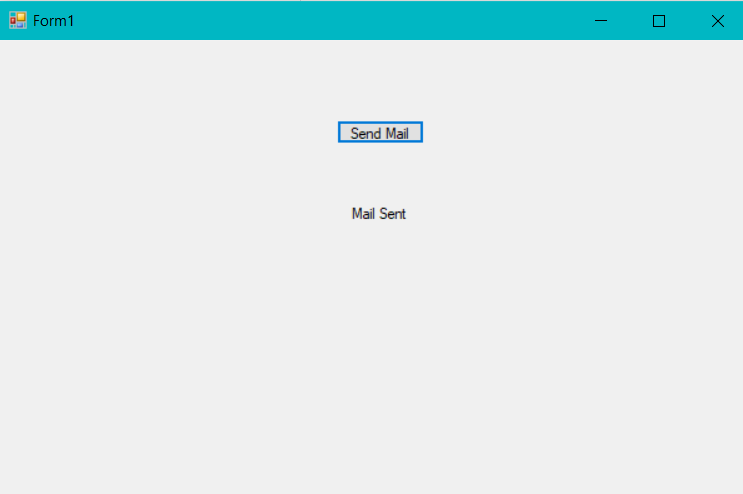
\includegraphics[width=4.27in]{10.png}\\
	 	\hfill\break\rule{6.27in}{1.2pt}
	 	\hfill\break\textbf{\emph{Thanks, Stay Hydrated and Keep Breathing.}}
	 \end{center}
\end{document}